% Options for packages loaded elsewhere
\PassOptionsToPackage{unicode}{hyperref}
\PassOptionsToPackage{hyphens}{url}
\PassOptionsToPackage{dvipsnames,svgnames,x11names}{xcolor}
%
\documentclass[
  11pt,
  letterpaper]{article}
\usepackage{amsmath,amssymb}
\usepackage{iftex}
\ifPDFTeX
  \usepackage[T1]{fontenc}
  \usepackage[utf8]{inputenc}
  \usepackage{textcomp} % provide euro and other symbols
\else % if luatex or xetex
  \usepackage{unicode-math} % this also loads fontspec
  \defaultfontfeatures{Scale=MatchLowercase}
  \defaultfontfeatures[\rmfamily]{Ligatures=TeX,Scale=1}
\fi
\usepackage{lmodern}
\ifPDFTeX\else
  % xetex/luatex font selection
\fi
% Use upquote if available, for straight quotes in verbatim environments
\IfFileExists{upquote.sty}{\usepackage{upquote}}{}
\IfFileExists{microtype.sty}{% use microtype if available
  \usepackage[]{microtype}
  \UseMicrotypeSet[protrusion]{basicmath} % disable protrusion for tt fonts
}{}
\makeatletter
\@ifundefined{KOMAClassName}{% if non-KOMA class
  \IfFileExists{parskip.sty}{%
    \usepackage{parskip}
  }{% else
    \setlength{\parindent}{0pt}
    \setlength{\parskip}{6pt plus 2pt minus 1pt}}
}{% if KOMA class
  \KOMAoptions{parskip=half}}
\makeatother
\usepackage{xcolor}
\usepackage[margin=1in]{geometry}
\usepackage{graphicx}
\makeatletter
\newsavebox\pandoc@box
\newcommand*\pandocbounded[1]{% scales image to fit in text height/width
  \sbox\pandoc@box{#1}%
  \Gscale@div\@tempa{\textheight}{\dimexpr\ht\pandoc@box+\dp\pandoc@box\relax}%
  \Gscale@div\@tempb{\linewidth}{\wd\pandoc@box}%
  \ifdim\@tempb\p@<\@tempa\p@\let\@tempa\@tempb\fi% select the smaller of both
  \ifdim\@tempa\p@<\p@\scalebox{\@tempa}{\usebox\pandoc@box}%
  \else\usebox{\pandoc@box}%
  \fi%
}
% Set default figure placement to htbp
\def\fps@figure{htbp}
\makeatother
\setlength{\emergencystretch}{3em} % prevent overfull lines
\providecommand{\tightlist}{%
  \setlength{\itemsep}{0pt}\setlength{\parskip}{0pt}}
\setcounter{secnumdepth}{5}
\usepackage[notextcomp]{kpfonts}
\usepackage{Inconsolata}
\usepackage{caption}
\usepackage{float}
\captionsetup*{labelfont={sc},textfont={it},labelsep={colon},justification=centering,singlelinecheck=true}
\usepackage{bookmark}
\IfFileExists{xurl.sty}{\usepackage{xurl}}{} % add URL line breaks if available
\urlstyle{same}
\hypersetup{
  pdfauthor={John Koo},
  pdfsubject={Week 1 Handout},
  colorlinks=true,
  linkcolor={Maroon},
  filecolor={Maroon},
  citecolor={Blue},
  urlcolor={blue},
  pdfcreator={LaTeX via pandoc}}

\title{\textsc{Week 1 Handout}}
\usepackage{etoolbox}
\makeatletter
\providecommand{\subtitle}[1]{% add subtitle to \maketitle
  \apptocmd{\@title}{\par {\large #1 \par}}{}{}
}
\makeatother
\subtitle{Gov 50 Data Science for the Social Sciences}
\author{John Koo}
\date{September 2, 2025}

\begin{document}
\maketitle

\section{Contact Info}\label{contact-info}

\begin{table}[!h]

\centering

\begin{tabular}{l}
  \textbf{John Koo} \\
  PhD Candidate, Department of Government \\ \\
  
  \textbf{Email} (preferred): \href{mailto:johnkoo@fas.harvard.edu}{johnkoo@fas.harvard.edu} \\
  \textbf{Slack}: @johnkoo (in the Harvard University workspace) \\
  \textbf{Office hours}: Tuesdays, 1:30pm to 3:30pm @ CGIS Cafe (sign-up: \href{https://jkoo.nl/meet}{jkoo.nl/meet}) \\ \\ 
  \textbf{Section materials}: \url{https://github.com/tanxpyox/gov50-sections-jk}
  
  \end{tabular}
\end{table}

\section{Where to get help?}\label{where-to-get-help}

\begin{itemize}
\item
  For tech assistance or help with homework: \textbf{Course
  Assistant-led Study Halls}

  \begin{quote}
  Study halls are a combination of office hours and drop-in tutoring
  sessions. Course assistants will hold a table usually at one of the
  house dining halls or common rooms and help students with assignments
  and course material. Study halls work best if you come as a group and
  work on the assignments on your own while you are there and ask for
  help from the CAs when you get stuck.
  \end{quote}

  \begin{quote}
  Schedule: TBA
  \end{quote}
\item
  For initial help with course content: ask on course Slack (accessible
  via Canvas sidebar) or sign up for my office hours
\item
  For perspective and inspiration: sign up for Scott's office hours
\end{itemize}

\section{Getting the most (grades) out of this
class}\label{getting-the-most-grades-out-of-this-class}

\begin{itemize}
\tightlist
\item
  Podcast and Article Responses (5\%) {[}one two-page doc every other
  week{]}
\item
  Problem Sets (20\%) {[}seven to eight in total{]}
\item
  Mid-term exam (20\%) {[}in-class, written, closed book{]}
\item
  Final exam (20\%) {[}in-class, written, closed book{]}
\item
  \emph{Final project} (25\%)
\end{itemize}

\newpage

Generic advice for maximising grades and efficiency

\begin{itemize}
\tightlist
\item
  Everything you learn should help you work towards the final project
  (which is the biggest chunk of your grades)

  \begin{itemize}
  \tightlist
  \item
    Take the project milestones seriously and do not wait until the last
    minute
  \end{itemize}
\item
  Problem sets

  \begin{itemize}
  \tightlist
  \item
    Low hanging fruits - don't miss them; Can reuse code in your
    projects
  \item
    It's OK to make mistakes (each p-set is 2--3\% of your final grade)
  \item
    Work with your study group; but write up your p-sets individually
  \item
    Start early, so you have time to get help
  \item
    Set aside a ``focus session'' every week to do the problem sets; do
    not mull over the p-set for the whole week
  \end{itemize}
\item
  AI allowed and encouraged, except in exams. Start learning how to use
  AI to debug your code.
\item
  Keep your code organised in your GitHub repository - you may need them
  in your final project
\end{itemize}

\section{Getting Started}\label{getting-started}

\begin{itemize}
\item
  Software: R, RStudio
\item
  Version control: Git and GitHub
\end{itemize}

\begin{figure}
\centering
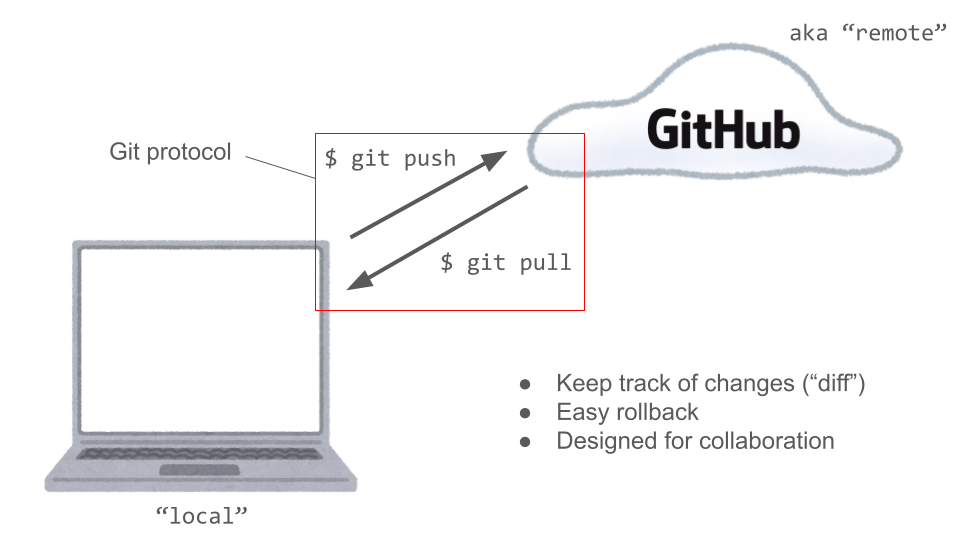
\includegraphics[width=0.75\linewidth,height=\textheight,keepaspectratio]{assets/gitvsgithub.png}
\caption{Git and GitHub}
\end{figure}

\section{Tasks}\label{tasks}

\begin{enumerate}
\def\labelenumi{\arabic{enumi}.}
\tightlist
\item
  Create an R project directory
\item
  Link it with Git
\item
  Publish the directory as a repository on GitHub
\item
  Making your first commit
\end{enumerate}

\end{document}
